% Preamble
\documentclass[11pt, a4paper]{article}
\usepackage[spanish]{babel}

% Packages
\usepackage{amsmath}
\usepackage[T1]{fontenc}
\usepackage{lmodern}
\usepackage{lipsum}
\usepackage{hyperref}
\usepackage{listings}
\usepackage{algorithm}
\usepackage{algpseudocode}
\usepackage{algorithmicx}
\usepackage{caption}
\usepackage{graphicx}
\usepackage{setspace}
\usepackage{float}

% Redefine caption label format
\captionsetup[algorithm]{labelsep=colon, name=Algoritmo}
\captionsetup{justification=centering}

% Document
\begin{document}

    \begin{titlepage}
        \begin{center}
            \begin{spacing}{1.5}
                \centering
                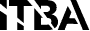
\includegraphics[width=0.2\textwidth]{./itba}
            \end{spacing}
            {\scshape\Large Instituto Tecnológico de Buenos Aires}
            {\rule{\textwidth}{0.4pt}}
            {\textbf{72.25 - Simulación de Sistemas}}
        \end{center}

        \vspace{35mm}

        \begin{center}
            \begin{spacing}{1.5}
                {\LARGE{\textbf{AUTÓMATAS CELULARES: BANDADAS DE AGENTES AUTOPROPULSADOS}}}
            \end{spacing}
        \end{center}

        \vspace{50mm}

        \begin{minipage}[t]{0.47\textwidth}
            \begin{center}
                {\textbf{Alejo Flores Lucey}}
                \\
                Legajo 62622
                \\
                {\href{mailto:afloreslucey@itba.edu.ar}{afloreslucey@itba.edu.ar}}
            \end{center}
        \end{minipage}
        \hfill
        \begin{minipage}[t]{0.47\textwidth}
            \begin{center}
                {\textbf{Nehuén Gabriel Llanos}}
                \\
                Legajo 62511
                \\
                {\href{mailto:nllanos@itba.edu.ar}{nllanos@itba.edu.ar}}
            \end{center}
        \end{minipage}

        \vspace{25mm}

        \begin{center}
            {\large{\textbf{2024 1C}}}
            \\
            {\large{Grupo Nº3}}
        \end{center}
    \end{titlepage}

    \tableofcontents
    \newpage

    \section{Introducción}
    \label{sec:introduccion}

        En el presente informe se presentará el análisis de la implementación computacional del modelo de un autómata
        Off Lattice, que busca representar el comportamiento de un sistema de partículas autopropulsadas en un espacio
        bidimensional.
        El estudio que se realiza a continuación se basa en el paper \textit{Novel Type of Phase Transition in a System
        of Self-Driven Particles} de \textit{Tamás Vicsek, András Czirók, Eshel Ben-jacob, Inon Cohen y Ofer Shochet},
        publicado en 1995.

        La implementación del modelo permite simular el sistema de partículas y definir observables que permiten
        estudiar el comportamiento del mismo en función de la variación de los parámetros de entrada.
        Por un lado, se estudiará el comportamiento del sistema en función de la cantidad de partículas y el ruido del
        mismo.
        Por otro lado, se analizará cómo las partículas atraviesan zonas circulares fijas en el espacio bidimensional,
        tanto en condiciones periódicas de contorno (PBC) como condiciones abiertas de contorno (OBC).
        En este sentido, se estudiarán los siguientes observables:

        \begin{itemize}
            \item Parámetro de orden del sistema.
            \item Tiempo en el que el número de visitas alcanza un dado porcentaje de la cantidad de partículas del sistema, para el caso de PBC\@.
            \item Número de visitas por unidad de tiempo, para el caso de OBC\@.
        \end{itemize}

        \subsection{Sistema Real}
        \label{subsec:sistema-real}

            El modelo Off Lattice busca analizar el movimiento de un conjunto de partículas cuando estas interactúan
            entre sí y como se produce un efecto de agrupamiento entre ellas a medida que el tiempo transcurre.
            Este fenómeno se lo conoce como movimiento colectivo en la naturaleza y es observado en comportamientos como
            el vuelo de bandadas de pájaros, el desplazamiento de cardúmenes de peces, entre otros.
            Además, se manifiesta a nivel microscópico en sistemas como el movimiento de bacterias y las células.

        \subsection{Fundamentos}
        \label{subsec:fundamentos}

            El sistema se puede caracterizar a través de tres parámetros de entrada, que determinarán el comportamiento
            del mismo:

            \begin{itemize}
                \item $N$: Cantidad de partículas.
                \item $L$: Longitud del lado del espacio bidimensional.
                \item $r_c$: Radio de interacción de las partículas.
                \item $\eta$: Ruido.
            \end{itemize}

            El modelo de Bandadas de Agentes Autopropulsados se basa en dos ecuaciones principales: la ecuación de la posición y la ecuación del ángulo de la velocidad.
            La primera de ellas:

            \begin{equation}
                x_i(t+1) = x_i(t) + v_i(t) \Delta t
            \end{equation}

            Donde $x_i(t)$ es la posición de la partícula i-ésima en el instante de tiempo $t$, $v_i(t)$ es la velocidad de la partícula i-ésima
            y $\Delta t$ es el paso de tiempo.
            Por otro lado, tenemos la segunda ecuación:

            \begin{equation}
                \theta(t+1) = \langle \theta(t) \rangle_r+ \Delta \theta
            \end{equation}

            Donde $\langle \theta(t) \rangle_r$ es el promedio de los ángulos de todas las partículas dentro de $r$ incluyendo la propia
            partícula, donde $r$ es el radio de interacción de la partícula, en el instante de tiempo $t$ y
            $\Delta \theta$ es el ruido uniforme entre $[-\eta/2, \eta/2]$.

            El promedio de los ángulos de las partículas vecinas se calcula de la siguiente manera:

            \begin{equation}
                \langle \theta(t) \rangle_r = atan2(\langle sin(\theta(t)) \rangle_r, \langle cos(\theta(t)) \rangle_r)
            \end{equation}

    \newpage

    \section{Implementación}
    \label{sec:implementacion}

        La implementación del modelo matemático de autómatas autopropulsados se realizó en Java, en su versión 19 en
        conjunto con Maven para la gestión de dependencias.

        Java se utilizó para la implementación del modelo Off Lattice, y para llevar adelante la simulación.
        Por otro lado, Python se utilizó para la creación de animaciones y el cálculo y visualización de los observables
        estudiados.

        Para iniciar el desarrollo de este modelo computacional, se partió del código realizado en el Trabajo Práctico Nro. 1 que
        implementaba el \textit{Cell Index Method} en Java.
        Este método permite obtener las partículas vecinas de una partícula en específico considerando un radio y un conjunto de celdas determinado.
        Esta implementación posibilita la obtención del ángulo que tendrá la partícula a analizar en específico luego de verse afectada por los ángulos de aquellas que se consideran vecinas.

        En el proyecto Java se tienen tres clases principales:

        La primera de ellas es \texttt{MovingParticle}, que extiende de la clase \texttt{Particle} y que representa a una
        partícula que se mueve en el espacio.
        \texttt{Particle} es una clase utilizada en el TP1 y que tiene como atributos el radio de la partícula, su posición en el eje $x$, su posición en el eje $y$ y un
        identificador. \texttt{MovingParticle} hereda todos los atributos mencionados previamente y cuenta con otros dos más que son
        el ángulo de la partícula y el módulo de su velocidad en un instante de tiempo.

        La segunda clase principal es \texttt{OffLatticeAutomata}, que representa el modelo de autómatas autopropulsados.
        La misma cuenta con dos atributos: el ruido que tiene el sistema y una instancia de la clase \texttt{CellIndexMethod} del TP1.
        El método principal de esta clase es \texttt{execute()} que se encarga de crear los archivos de salida que contienen la información de las partículas del sistema
        en cada instante de tiempo teniendo en cuenta los parámetros de entrada del modelo: $N$ (cantidad de partículas), $L$ (longitud
        del lado del espacio bidimensional), $r_c$ (radio de interacción), $v$ (módulo de la velocidad de las partículas), $\eta$ (ruido) y
        $t$ (la cantidad de instantes que se quieren simular).

        Por último, la tercera clase principal es \texttt{Main}.
        Esta se encarga de leer los parámetros de entrada de un archivo input y realizar la ejecución del modelo de
        autómatas autopropulsados.
        Con la información de las partículas obtenidas en los archivos output que se generan en este programa, se pueden generar las animaciones y llevar a cabo el estudio de los observables.

        \subsection{Arquitectura}
        \label{subsec:arquitectura}

            La arquitectura del código implementado se puede observar en la Figura~\ref{fig:architecture}.
            En la misma se puede ver que el programa principal \texttt{Main} se encarga de leer los parámetros de entrada
            y ejecutar el modelo de autómatas autopropulsados.

            Vale la pena mencionar que se decidió utilizar el patrón \textit{Builder} para la instanciación de las clases.
            Esto permite que la creación de las mismas sea más sencilla y autodescriptiva.
            Asimismo, permite la reutilización de código de manera rápida y simple y la creación de objetos con
            múltiples atributos de manera más clara.

            \begin{figure}[htbp]
                \centering
                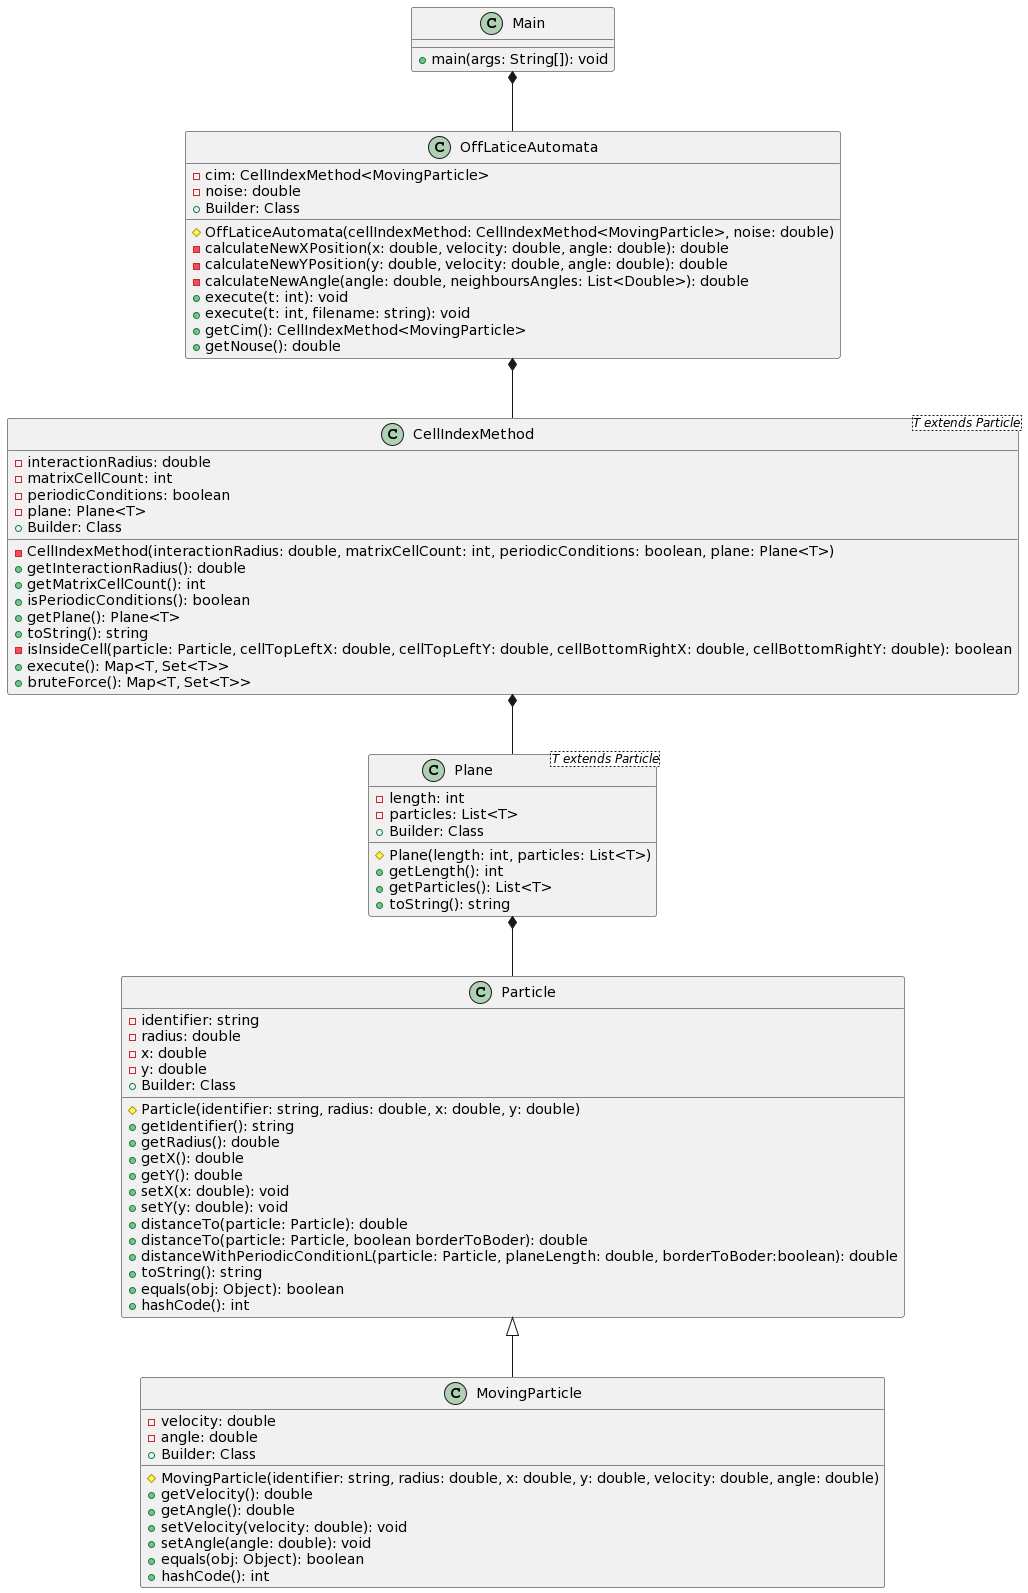
\includegraphics[height=0.69\textheight]{./architecture}
                \caption{Arquitectura del código implementado.}
                \label{fig:architecture}
            \end{figure}

        \subsection{Algoritmo}
        \label{subsec:algoritmo}

            La simulación del modelo de autómatas autopropulsados se basa en las dos funciones principales descritas en la sección
            de Fundamentos.
            A continuación, se presenta el modelo computacional en pseudocódigo que se ha implementado.
            Véase el Algoritmo~\ref{alg:algorithm}.

            \begin{algorithm}
                \caption{Autómata Off Lattice}
                \begin{algorithmic}[1]
                    \State Se crea una archivo de salida para la simulación
                        \While{$t < t_{max}$}
                            \State Ejecución de CellIndexMethod
                            \State Obtención de las partículas vecinas de cada partícula en $t$
                            \State Creación de una lista de objetos Partícula - ÁngulosVecinas en $t$
                            \For{Par en lista de Partícula - ÁngulosVecinas}
                                \State Cálculo del ángulo promedio de las partículas vecinas
                                \State Definición del nuevo ángulo de la partícula en $t+1$
                                \State Actualización de la posición en $x$ de la partícula en $t+1$
                                \State Actualización de la posición en $y$ de la partícula en $t+1$
                                \State Escritura de la información de la partícula en archivo output
                            \EndFor
                            \State Incremento del instante de tiempo $t$
                        \EndWhile
                \end{algorithmic}
                \label{alg:algorithm}
            \end{algorithm}

            Una observación importante a tener en cuenta es que el \texttt{CellIndexMethod} retorna un mapa, es decir, una estructura
            que está conformada por una clave y un valor.
            En este caso, la clave es una partícula y el valor es una lista con todas las partículas vecinas de la misma.
            Otro aspecto relevante a mencionar es que la lista formada por objetos del tipo Partícula - ÁngulosVecinas
            tiene copias y no referencias de los ángulos correspondientes a las partículas vecinas.
            Esto es así para evitar que la actualización de un ángulo se vea afectada por la actualización de otro
            ángulo en el mismo instante de tiempo.

    \newpage

    \section{Simulaciones}
    \label{sec:simulaciones}

        En esta sección se describirá el sistema particular que se va a simular y estudiar. Para ello, se
        presentarán aspectos como la geometría, el rango de parámetros fijos y variables, los inputs y outputs
        y se definirán los observables que se calcularán a partir del output de la simulación.

        Se ha decidido mantener fijos los siguientes parámetros en todas las simulaciones, siguiendo los parámetros utilizados en el paper de referencia:
        \begin{itemize}
            \item $r_c = 1$
            \item $v = 0,03$
            \item $L = 5$
        \end{itemize}

        Las simulaciones realizadas buscan obtener resultados sobre como determinados observables escalares varían
        en función de los parámetros de entrada variables.
        Aquellos observables a analizar son:
        \begin{itemize}
            \item Parámetro de Orden: $v_a$.
            \item Tiempo en el que el número de visitas alcanza un dado porcentaje de N, para las visitas con condiciones periódicas de contorno (PBC).
            \item Número de visitas por unidad de tiempo, para las visitas con condiciones abiertas de contorno (OBC).
        \end{itemize}

        Los parámetros variables son:

        \begin{itemize}
            \item $N$: Cantidad de partículas.
            \item $\eta$: Ruido.
        \end{itemize}

        A continuación se describirá el sistema particular elegido para cada observable escalar a estudiar.

        \subsection{Parámetro de Orden o Polarización ($v_a$)}
        \label{subsec:polarizacion}

            Este primer observable escalar se define como:

            \begin{equation}
                v_a = \frac{1}{Nv} \left|\sum_{i=1}^{N} \vec{v_i} \right|
            \end{equation}

            Donde $N$ representa la cantidad de partículas y $v$ es el módulo de la velocidad de las mismas.
            Por último, se tiene la norma de la sumatoria de todos los vectores $\vec{v_i} \ / \  0 \geq i < N$,
            que representan el vector velocidad de la partícula i-ésima.
            El valor del parámetro de orden tiende a cero (0) cuando las partículas se encuentran en total desorden;
            por otro lado, tiende a uno (1) cuando las partículas se encuentran polarizadas, es decir, se trasladan en la misma dirección.

        \subsection{Visitas PBC: tiempo en el que el número de visitas alcanza un dado porcentaje de N.}
        \label{subsec:visitas-pbc}

            En este caso, luego de ejecutar la simulación de un sistema de partículas que se mueven en una celda de lado $L$,
            se estudia cómo las partículas circulan a través de cuatro (4) zonas de conteo circulares fijas de radio $0,5$.
            Su ubicación, si bien es calculada aleatoriamente, se mantiene constante para todas las simulaciones, cuando se varía $N$ 0 $\eta$.

            Al tener condiciones periódicas de contorno, se consideran que los identificadores de las partículas son inmutables.
            Por lo tanto, cada partícula solo debe ser contabilizada una vez al visitar cada zona de medición.
            El observable a estudiar es el tiempo en el que el número de visitas alcanza el 20\% de N dependiendo
            del $\eta$ (ruido).

            Este estudio se realiza para cuatro (4) Ns distintos ($100$, $300$, $500$ y $1000$) y para cada uno de ellos
            se varía $\eta$ en un rango de $0$ a $5,8$ con un paso de $0,2$.

            Resulta interesante analizar el método de obtención de los resultados para cada simulación, puesto que se
            tienen cuatro (4) zonas circulares fijas ubicadas en lugares distintos.
            En consecuencia, para poder el obtener el valor del observable, primero se deben promediar los tiempos obtenidos
            de cada una de las zonas de conteo.
            Dicho cálculo se realiza de la siguiente manera:

            \begin{equation}
                t_{\text{prom}} = \frac{1}{4} \sum_{i=1}^{4} t_i \ ,\ t_i\text{: tiempo en la zona }i
            \end{equation}
            Al ser un promedio entre cuatro (4) valores, es necesario calcular el error mediante desvío estándar.
            Al ser un tamaño de muestra pequeño, se introduce un sesgo en la estimación de la desviación estándar. Dicho sesgo se corrige limitando los grados de libertad en 1, es decir, \texttt{ddof=1}:

            \begin{equation}
                \sigma = \sqrt{\frac{1}{3} \sum_{i=1}^{4} (t_i - t_{\text{prom}})^2}
            \end{equation}

            Con estos dos valores obtenidos se obtendrá el valor del observable y su error en función del $\eta$ para cada $N$ de los mencionados previamente.

        \subsection{Visitas OBC: número de visitas por unidad de tiempo.}
        \label{subsec:visitas-obc}

            El sistema que se simula en este caso es el mismo que se describe en el primer apartado de la subsección
            anterior, pero con la particularidad de que ahora se realiza con condiciones abiertas de contorno.
            Esta condición refiere al hecho de que los identificadores de las partículas no se considerarán inmutables.
            Esto significa que, a la hora de reingresar a las zonas de conteo, una misma partícula será contabilizada nuevamente.

            El observable a estudiar es el número de visitas por unidad de tiempo dependiendo de $\eta$ (ruido), es decir,
            la pendiente de la curva número de visitas en función del tiempo en la zona donde dicho valor sea estacionario.
            Este estudio, al igual que el descripto en el apartado anterior, se realiza para los mismos cuatro (4) Ns
            ($100$, $300$, $500$ y $1000$), variando $\eta$ en el mismo rango (de $0$ a $5,8$, con un paso de $0,2$).

            Como el objetivo es obtener la pendiente de la curva número de visitas en función del tiempo, es necesario obtener las curvas
            de cada una de las cuatro (4) zonas de conteo.
            Dado que el caracter de estas curvas es no lineal, es imperioso obtener la pendiente de la recta asociada
            a cada una de ellas mediante el método de regresión lineal simple, que es un método que permite aproximar
            la relación de dependencia entre una variable independiente $y$ (cantidad de visitas) y un conjunto de
            variables independientes $x$ (tiempo).
            La definición de la recta asociada es la siguiente:

            \begin{equation}
                y = \beta_0 x + \beta_1
            \end{equation}

            Como se puede observar, existen dos coeficientes $\beta_0$ y $\beta_1$ que no se conocen.
            Como para el estudio que se está realizando solamente es de interés la pendiente, se puede obviar el cálculo
            de $\beta_1$ y obtener directamente el valor de $\beta_0$ con la siguiente fórmula:

            \begin{equation}
                \beta_0 = \frac{N \sum_{i=1}^N x_i y_i - \sum_{i=1}^N x_i \sum_{i=1}^N y_i }{N \sum_{i=1}^N x_i^2 - \left(\sum_{i=1}^N x_i \right)^2}
            \end{equation}

            Este coeficiente representa el valor de la pendiente de la recta asociada a la curva de visitas en función de tiempo y
            debido a que es una pendiente, de ahora en más se la llamará $m$:

            \begin{equation}
                m_k = \frac{N \sum_{i=1}^N x_i y_i - \sum_{i=1}^N x_i \sum_{i=1}^N y_i }{N \sum_{i=1}^N x_i^2 - \left(\sum_{i=1}^N x_i \right)^2}
                \ , 1 \leq k \leq 4
            \end{equation}

            En el numerador se tiene a la diferencia entre el producto entre $N$ y la sumatoria de las variables dependientes e independientes
            y la sumatoria de los productos de las variables independientes y dependientes.
            Por otro lado, en el denominador se tiene a la diferencia entre el producto entre $N$ y la sumatoria de los
            cuadrados de las variables independientes y el cuadrado de la sumatoria de las variables independientes.
            $k$ representa la zona de conteo a la que se le está calculando la pendiente.

            Para poder obtener un valor único del observable, es necesario obtener el promedio de las pendientes de las cuatro (4) zonas:

            \begin{equation}
                m_{prom}(N,\eta) = \frac{1}{4} \sum_{i=1}^{4} m_i
            \end{equation}

            Además, por su condición de promedio debemos obtener el error asociado mediante el desvío estándar.
            Como fue mencionado anteriormente, al ser un tamaño de muestra pequeño, se introduce un sesgo en la estimación de la desviación estándar. Dicho sesgo se corrige limitando los grados de libertad en 1, es decir, \texttt{ddof=1}:

            \begin{equation}
                \sigma = \sqrt{\frac{1}{3} \sum_{i=1}^{4} (m_i - m_{prom})^2}
            \end{equation}

            Con estas consideraciones podremos obtener los diferentes valores del observable y su error en función de $\eta$
            para cada $N$ de los mencionados previamente.

    \newpage

    \section{Resultados}
    \label{sec:resultados}

        En esta sección se presentarán los resultados obtenidos de las simulaciones realizadas.
        Para cada uno de los observables estudiados se mostrarán animaciones características del sistema,
        figuras del observable en función del tiempo y figuras del observable en función de $\eta$.

        \subsection{Parámetro de Orden o Polarización ($v_a$)}
        \label{subsec:resultados-polarizacion}

            En la Figura~\ref{fig:parametro_orden_1} se podrá observar un fotograma de la animación característica del sistema, en donde,
            la densidad $\rho$ es igual a sesenta (12), el ruido $\eta$ es de dos coma cuatro (2,4) y la cantidad de partículas $N$ es de 300.

            \begin{figure}[H]
                \centering
                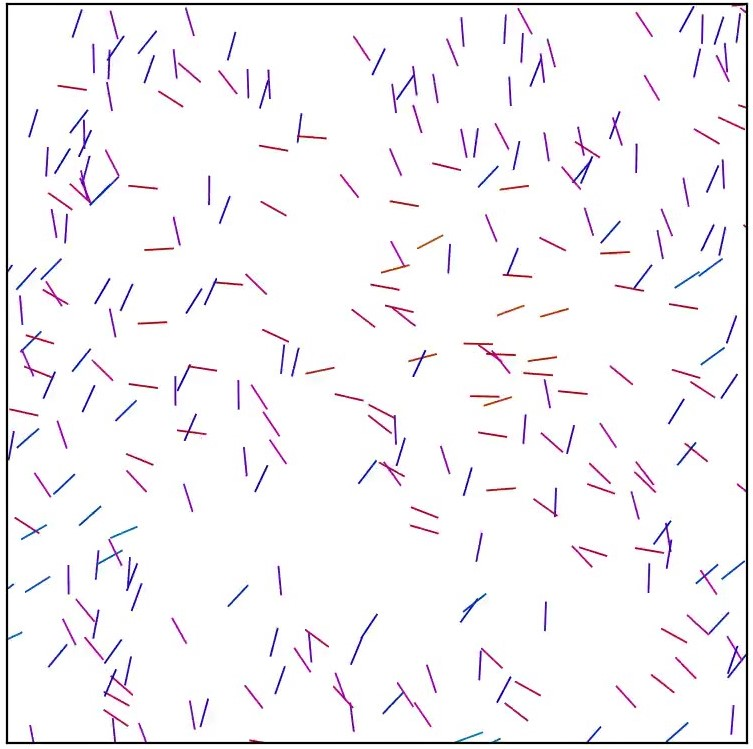
\includegraphics[width=\textwidth]{./animation-n300-eta2p4-frame}
                \caption{Fotograma de la animación con 300 partículas, $\eta = 2.4$ y $\rho = 12$.\\Véase la animación completa \href{https://youtu.be/aZ9eOtlXgQw}{aquí}.}
                \label{fig:parametro_orden_1}
            \end{figure}

            Se puede observar que las partículas tienden a moverse en dos direcciones preferenciales, lo que indica que
            el sistema se encuentra algo polarizado.

            En la Figura~\ref{fig:parametro_orden_2} se muestra el parámetro de orden en función del tiempo para diferentes valores de $\eta$
            y un $N$ igual a trescientos (300).
            Se puede visualizar que a medida que el ruido aumenta, la polarización adquiere valores estacionarios cada
            vez más bajos y una variación más pronunciada.

            También se puede destacar el hecho de que, en todos los casos, el observable tiende a un comportamiento
            estacionario a medida que el tiempo transcurre.

            \begin{figure}[H]
                \centering
                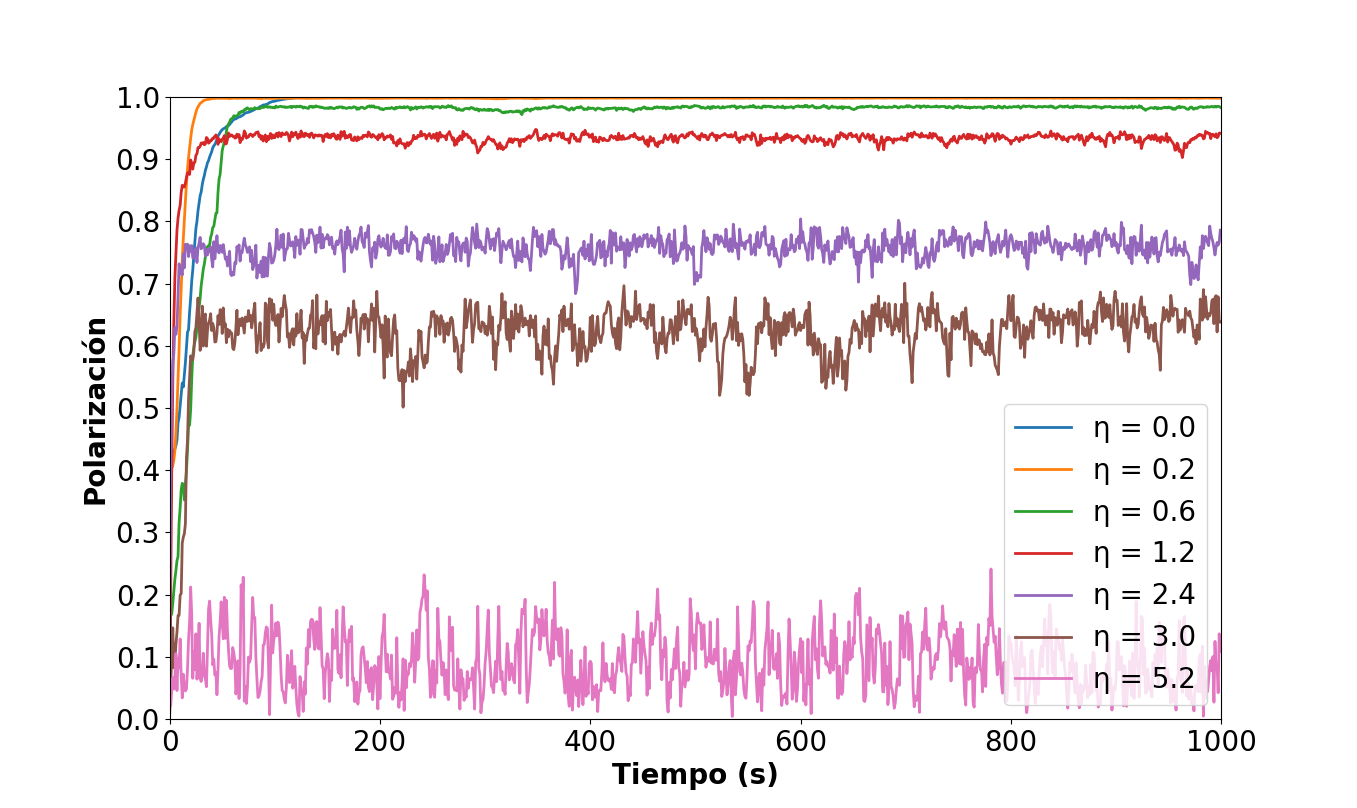
\includegraphics[width=\textwidth]{./va_vs_time-n300}
                \caption{Polarización en función del tiempo para $N = 300$ y diferentes valores de $\eta$.}
                \label{fig:parametro_orden_2}
            \end{figure}

            Por último, en la Figura~\ref{fig:parametro_orden_3}, que se muestra a continuación, se puede observar el
            promedio del parámetro de orden en el estado estacionario en función del ruido $\eta$ para tres valores de
            $N$ distintos: $300$, $500$ y $1000$.
            Asimismo, se pueden ver las barras de error asociadas a los diferentes valores del observable.
            Véase la sección~\ref{subsec:polarizacion} para un análisis más detallado del cálculo de dichos valores.

            \begin{figure}[H]
                \centering
                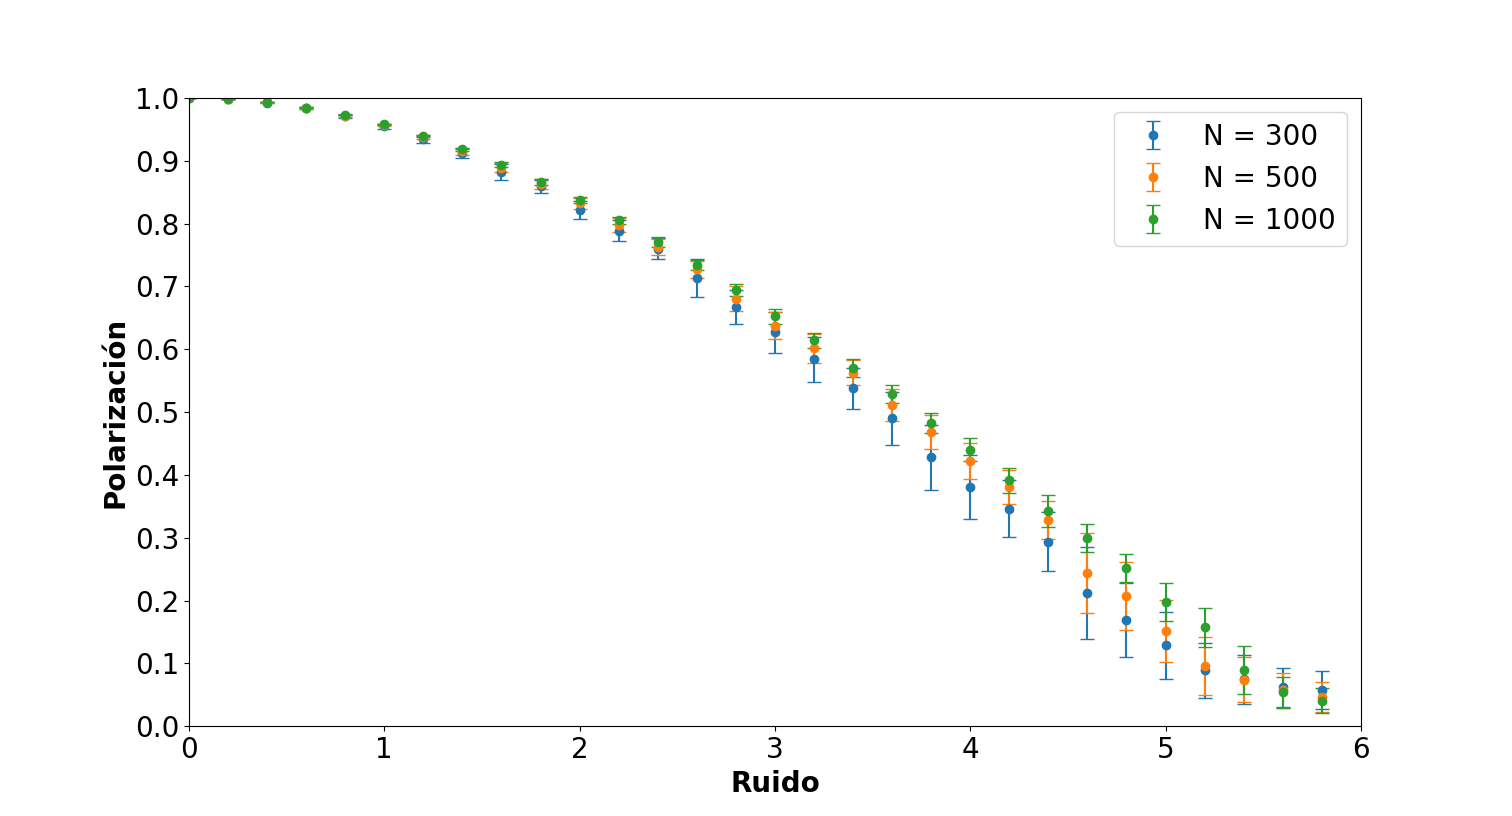
\includegraphics[width=\textwidth]{./va_vs_eta}
                \caption{Polarización promedio en estado estacionario en función del ruido $\eta$ para $N=300$, $N=500$ y $N=1000$.}
                \label{fig:parametro_orden_3}
            \end{figure}

            Analizando la Figura~\ref{fig:parametro_orden_3} y comparando los valores del observable para cada uno de los $N$s, podemos deducir que
            cuando $N$ es mayor, los valores de la polarización son mayores.
            Además, se puede notar que el error asociado al observable disminuye a medida que $N$ aumenta, es decir, a
            medida que la muestra es mayor, el error asociado es menor.

            Como último comentario, se evidencia un incremento del error para los valores de $\eta$ que oscilan tres (3) y cinco (5).
            La teoría es que estos valores de $\eta$ no son ni muy cercanos al mínimo ni tampoco al máximo, lo que genera que
            la polarización varíe en un rango de valores amplio en el estado estacionario y, por lo tanto, genere un error
            mayor.
            Esta fluctuación de valores significativa se puede ver en la Figura~\ref{fig:parametro_orden_2} para el valor de $\eta = 3$ y
            $\eta = 5.2$; cuando el ruido es cercano a los extremos, el rango de variación para la polarización es menor y por
            consiguiente, el error también lo es.

        \subsection{Visitas PBC: tiempo en el que el número de visitas alcanza un dado porcentaje de N.}
        \label{subsec:resultados-visitas-pbc}

            En la Figura~\ref{fig:visitas_pbc_1} se muestra un fotograma de la animación característica del sistema, en donde
            el número de partículas $N$ es igual a trescientos (300), la longitud del plano $L$ es 5 y el ruido $\eta$ es 0,6.
            En la misma se pueden observar las partículas, como así también las zonas circulares fijas en las que se contabilizan las visitas.
            Las partículas que se encuentran en la zona de conteo son coloreadas de color verde.

            \begin{figure}[H]
                \centering
                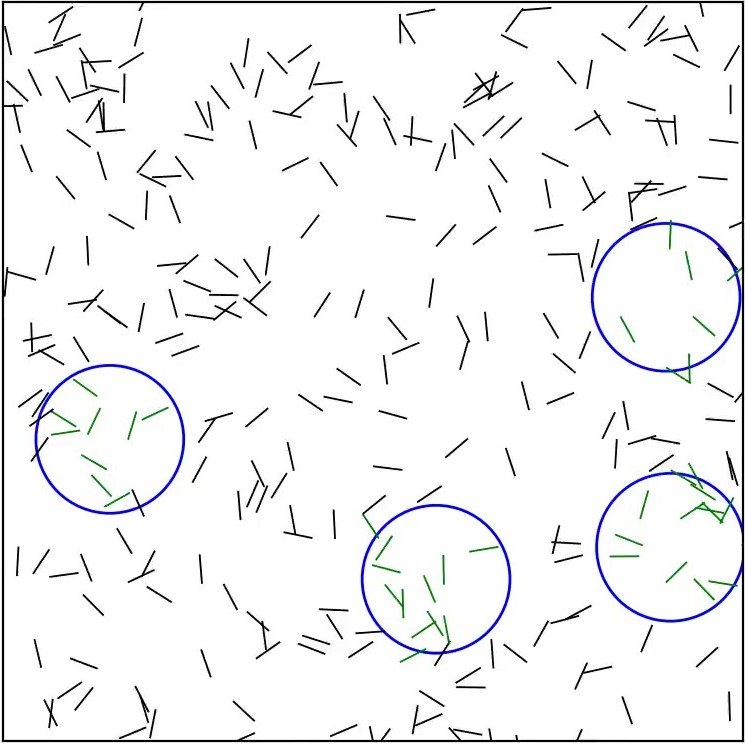
\includegraphics[width=\textwidth]{./animation_visits_pbc-n300-eta0p6-frame}
                \caption{Fotograma de la animación de visitas con condiciones periódicas de contorno con $300$ partículas, $L = 5$ y $\eta = 0.6$.\\Véase la animación completa \href{https://youtu.be/MGHMlVLz0Ys}{aquí}.}
                \label{fig:visitas_pbc_1}
            \end{figure}

            En la Figura~\ref{fig:visitas_pbc_2} se muestra el número de visitas totales en función del tiempo.
            Se pueden visualizar cuatro curvas, cada una correspondiente a una zona de conteo.

            \begin{figure}[H]
                \centering
                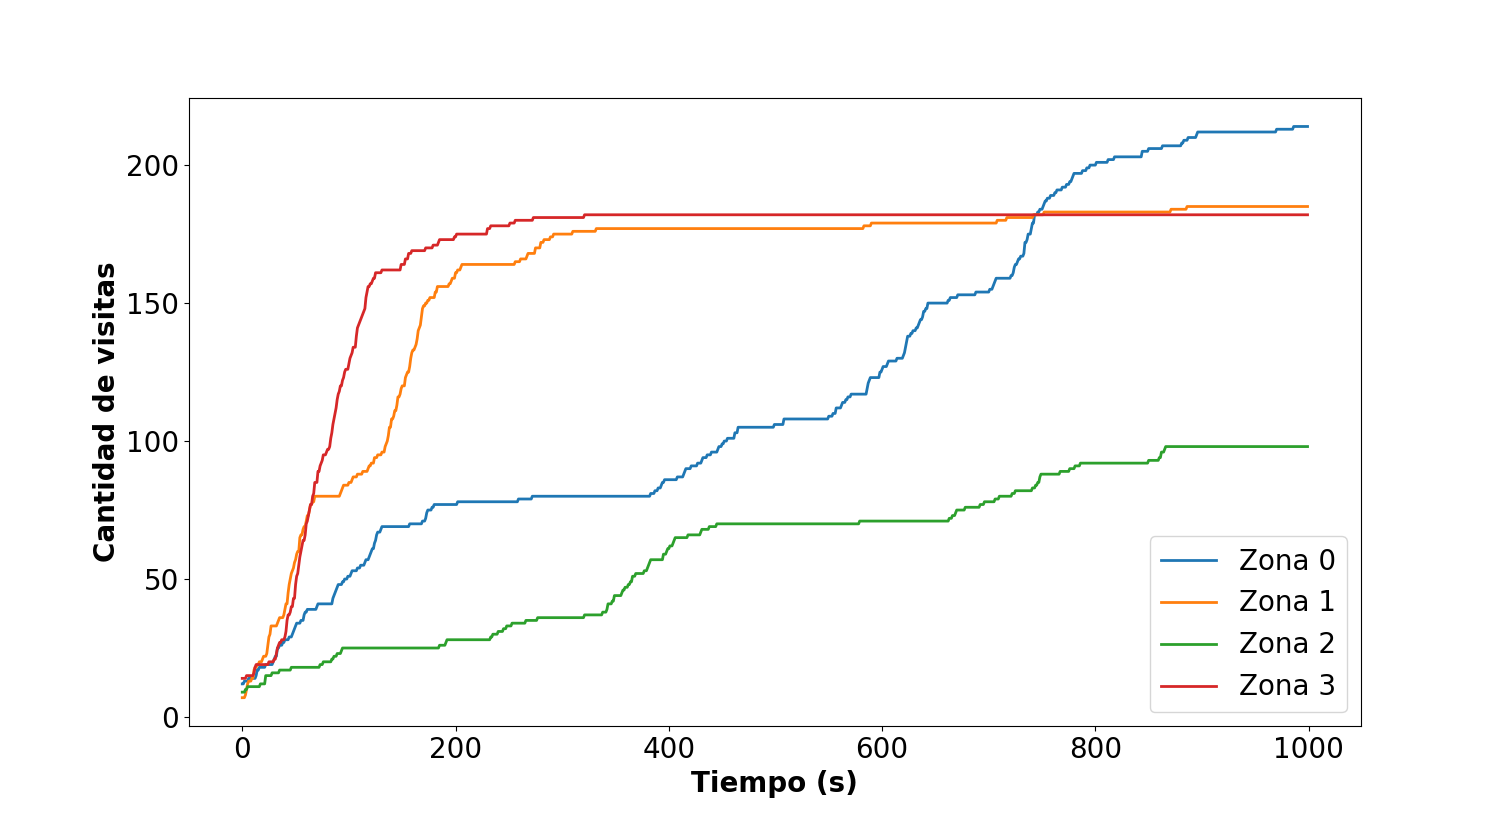
\includegraphics[width=\textwidth]{./visits_vs_time_pbc-n300-eta0p6}
                \caption{Cantidad de visitas totales en función del timepo, para $N = 300$, $L = 5$ y $\eta = 0.6$}
                \label{fig:visitas_pbc_2}
            \end{figure}

            Se puede observar que las curvas no varían de forma uniforme, sino que depende de la ubicación de las zonas de conteo.
            Asimismo, podemos señalar que el número de visitas llega a un máximo y luego se mantiene constante; esto se
            podría deber a que las partículas alcanzan un estado polarizado y ya han sido contabilizadas en esa zona.

            Por último, en la Figura~\ref{fig:visitas_pbc_3} se muestra el tiempo en el que el número de visitas alcanza
            el 20\% de $N$ en función de $\eta$ para diferentes valores de $N$.

            Se puede visualizar que a medida que el ruido aumenta, el tiempo en el que el número de visitas alcanza
            el 20\% de N también se incrementa.
            Además, se puede observar que el tiempo en el que el número de visitas alcanza el 20\% de N es menor a medida que $N$ aumenta.

            \begin{figure}[H]
                \centering
                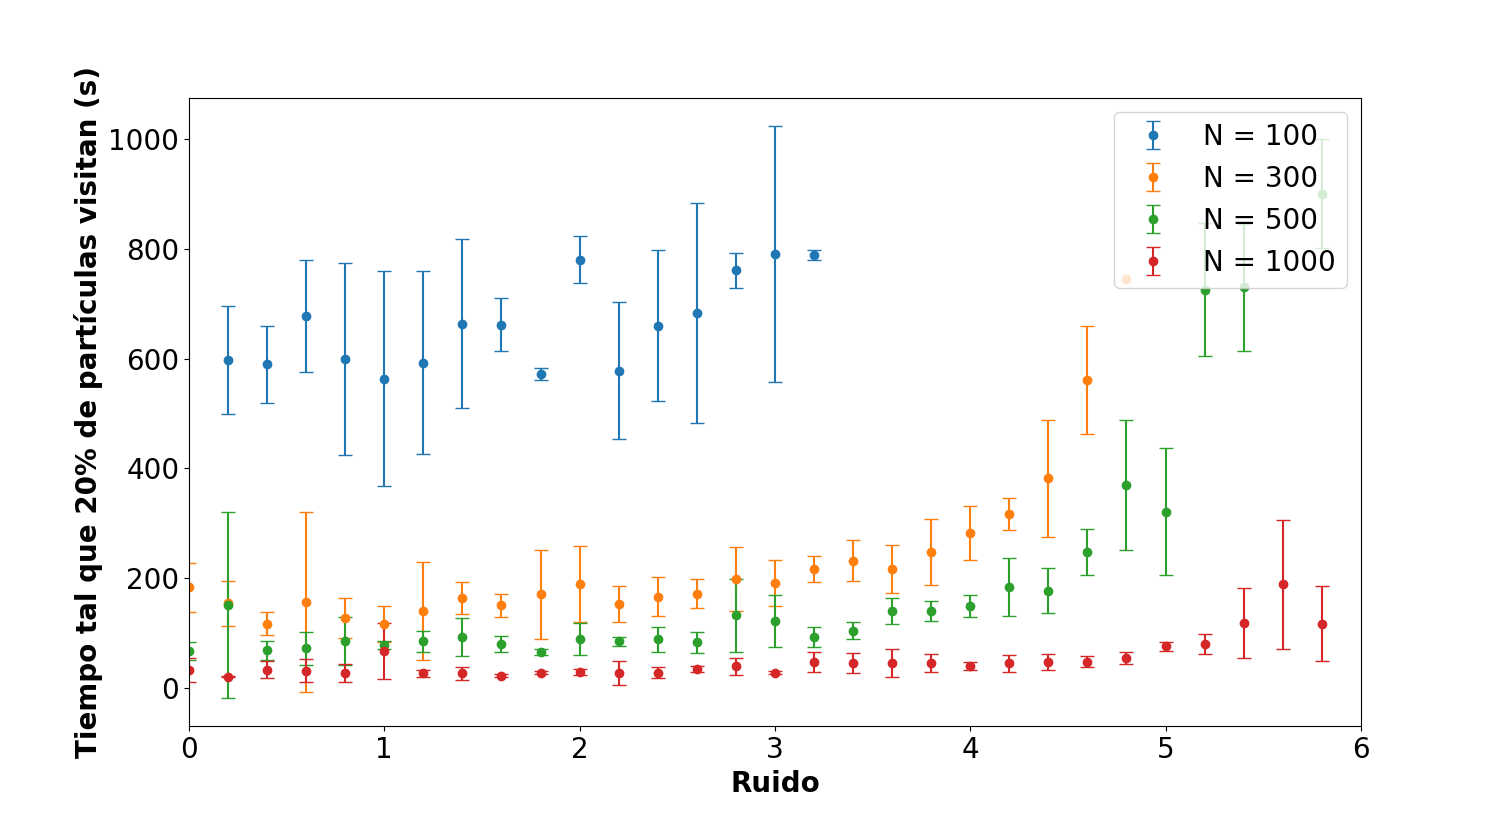
\includegraphics[width=\textwidth]{./threshold_vs_eta-pbc}
                \caption{Tiempo en el que el número de visitas alcanza el 20\% de N en función de $\eta$ para diferentes valores de $N$}
                \label{fig:visitas_pbc_3}
            \end{figure}

            Cabe mencionar que para ciertos valores de $N$ y $\eta$, no se alcanza el umbral del 20\% de $N$ en el tiempo de simulación.
            Esto se debe al desorden de las partículas, y su poca cantidad.

        \subsection{Visitas OBC: número de visitas por unidad de tiempo.}
        \label{subsec:resultados-visitas-obc}

            En la Figura~\ref{fig:visitas_obc_1} se muestra un fotograma de la animación característica del sistema, en donde
            el número de partículas $N$ es igual a trescientos (300), la longitud del plano $L$ es 5 y el ruido $\eta$ es 0,6.
            Al igual que en la sección anterior, en la misma se pueden observar las partículas, como así también las
            zonas circulares fijas en las que se contabilizan las visitas.
            Las partículas que se encuentran en la zona de conteo son coloreadas de color verde.

            \begin{figure}[H]
                \centering
                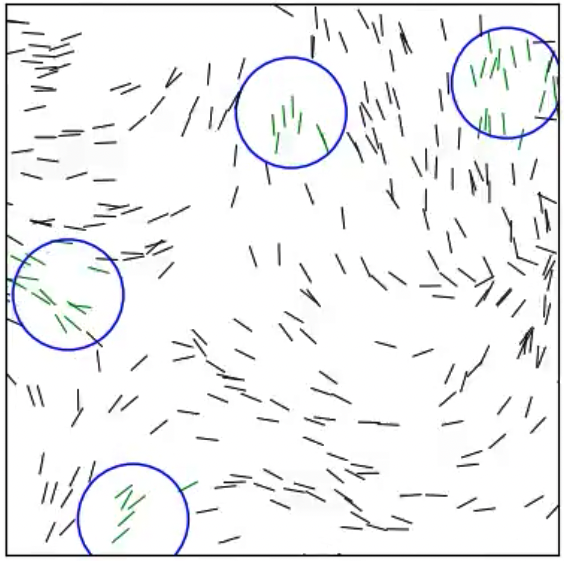
\includegraphics[width=\textwidth]{./animation_visits_obc-n300-eta0p6-frame}
                \caption{Fotograma de la animación de visitas con condiciones abiertas de contorno con $300$ partículas, $L = 5$ y $\eta = 0.6$.\\Véase la animación completa \href{https://youtu.be/TXe88VVMnL4}{aquí}.}
                \label{fig:visitas_obc_1}
            \end{figure}

            En la Figura~\ref{fig:visitas_obc_2} se muestra el número de visitas totales en función del tiempo.
            Se pueden visualizar cuatro curvas, cada una correspondiente a una zona de conteo.

            \begin{figure}[H]
                \centering
                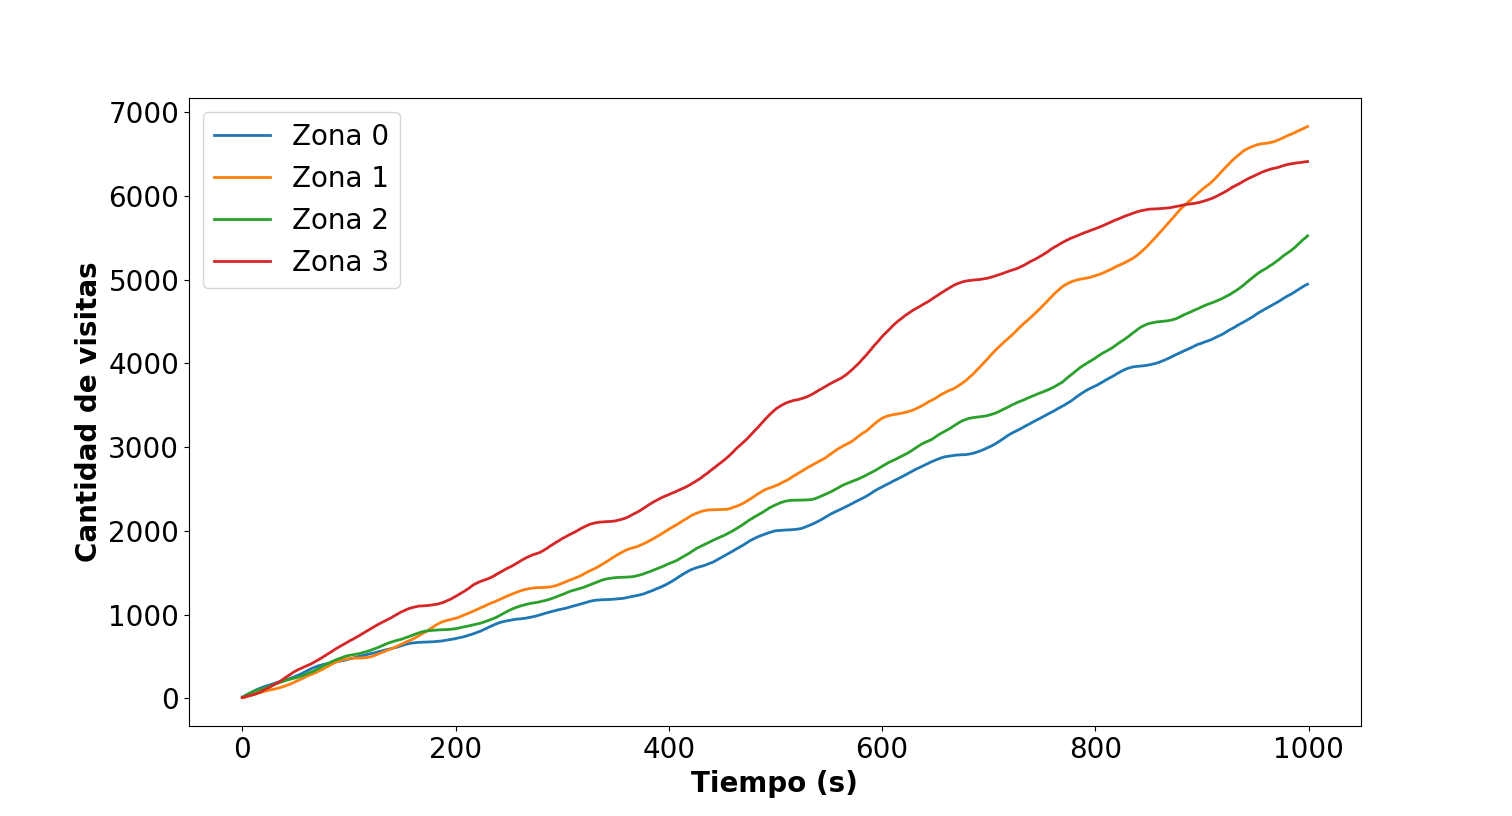
\includegraphics[width=\textwidth]{./visits_vs_time_obc-n300-eta0p6}
                \caption{Cantidad de visitas totales en función del timepo, para $N = 300$, $L = 5$ y $\eta = 0.6$}
                \label{fig:visitas_obc_2}
            \end{figure}

            Se puede observar que las curvas no varían de forma uniforme, sino que depende de la ubicación de las zonas de conteo.
            Sin embargo, se logra notar que el número de visitas totales se mantiene en constante crecimiento.
            Es por esta razón que resulta imposible utilizar el tiempo como observable escalar, y se debe recurrir a una
            métrica derivada de la misma; en este caso, la pendiente de la recta característica asociada a la curva.

            En la Figura~\ref{fig:visitas_obc_3} se muestra el número de visitas por unidad de tiempo en función de
            $\eta$ para diferentes valores de $N$.

            \begin{figure}[H]
                \centering
                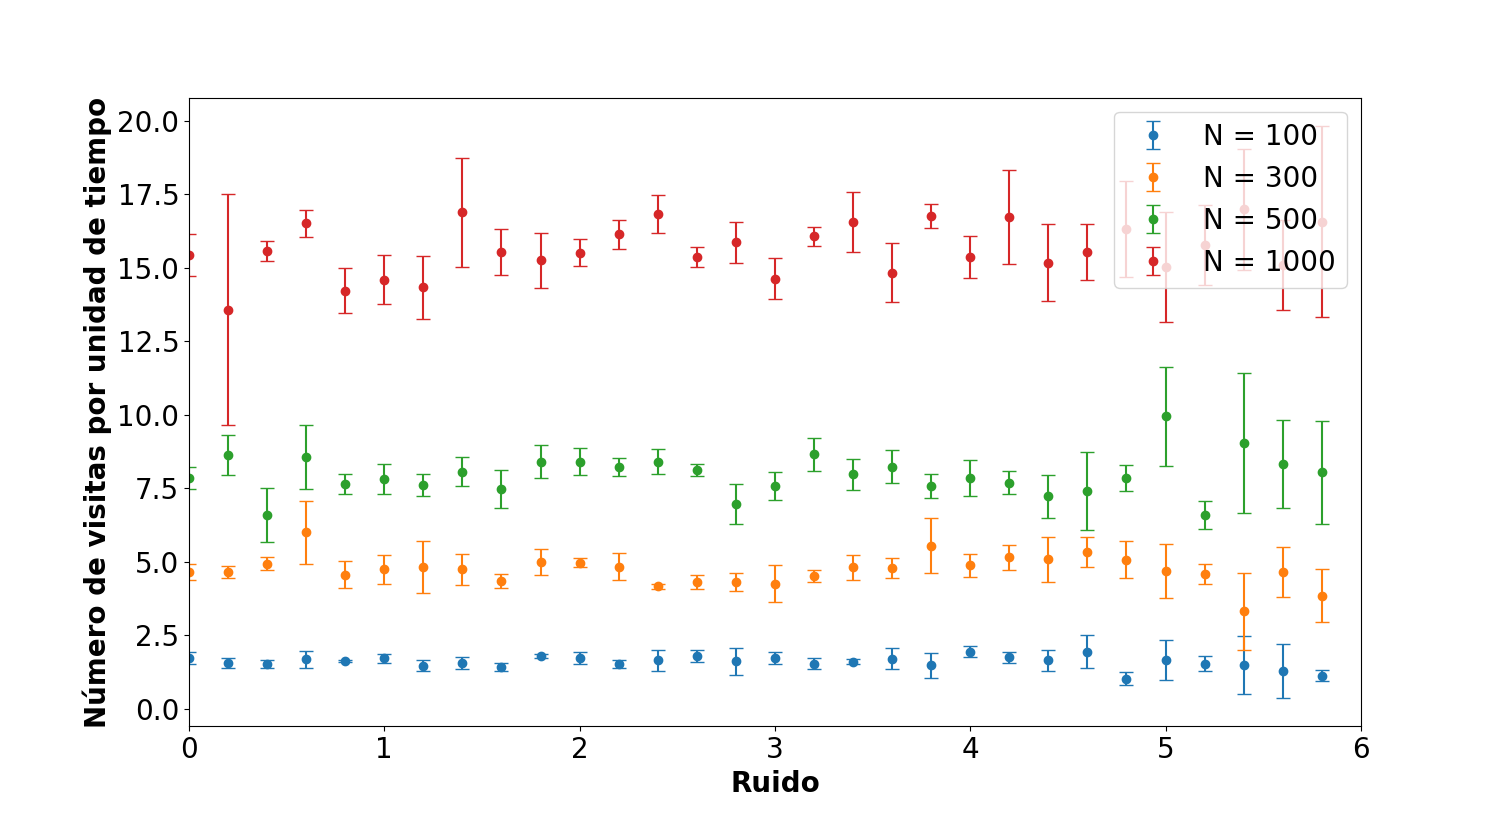
\includegraphics[width=\textwidth]{./slope_vs_eta-obc}
                \caption{Número de visitas por unidad de tiempo en función de $\eta$ para diferentes valores de $N$}
                \label{fig:visitas_obc_3}
            \end{figure}

            Cabe mencionar que la pendiente de la recta asociada a la curva de visitas en función del tiempo es un
            observable con un error asociado, pues se debe utilizar el método de regresión lineal simple para aproximar
            la curva a una recta.
            Véase la sección~\ref{subsec:visitas-obc} para un análisis más detallado del cálculo de dichos valores.

            Resulta particularmente interesante el resultado del gráfico de la Figura~\ref{fig:visitas_obc_3}.
            Se puede observar que a medida que el ruido aumenta, la cantidad de visitas por unidad de tiempo se mantiene
            en un rango de valores acotado constante.
            Además, se puede notar que la cantidad de visitas por unidad de tiempo es mayor a medida que $N$ aumenta,
            como es de esperar.

    \newpage

    \section{Conclusiones}
    \label{sec:conclusiones}

        En el presente informe se ha presentado la implementación computacional de un modelo de autómatas autopropulsados
        Off Lattice, que busca representar el comportamiento de un sistema de partículas autopropulsadas en un espacio
        bidimensional.
        Se ha estudiado el comportamiento del sistema en función de la cantidad de partículas y el ruido del mismo, así como
        también cómo las partículas atraviesan zonas circulares fijas en el espacio bidimensional, tanto en condiciones
        periódicas de contorno (PBC) como condiciones abiertas de contorno (OBC).

        Para el estudio de la polarización del sistema en función del ruido proporcionado, se concluye que a medida que
        el ruido aumenta, el parámetro de orden del sistema disminuye, lo que indica que las partículas se encuentran en
        un estado de mayor desorden.
        Resultó interesante estudiar la respuesta de la polarización ante valores de ruido cercanos al centro del
        intervalo, donde se puede examinar un comportamiento más errático y fluctuante del observable.
        Por último, se observó que a medida que aumenta la cantidad de partículas, la polarización tiende a ser
        levemente mayor.

        Por otro lado, para el estudio de las visitas en condiciones periódicas de contorno, se ha observado que el
        tiempo en el que el número de visitas alcanza un dado porcentaje de la cantidad de partículas del sistema aumenta
        a medida que el ruido aumenta.
        Asimismo, se pudo notar que para valores de baja cantidad de partículas y/o alto ruido, no se alcanza el umbral.

        Por último, para el estudio de las visitas en condiciones abiertas de contorno, se ha observado que la cantidad
        de visitas por unidad de tiempo se mantiene constante a medida que el ruido aumenta, sin importar la cantidad de
        partículas del sistema.
        Se ha encontrado que la cantidad de visitas por unidad de tiempo es mayor a medida que la cantidad de partículas
        aumenta, como es esperable debido al incremento de la densidad del sistema.

        Estas conclusiones reflejan los hallazgos y las observaciones derivadas del análisis de los resultados
        obtenidos de la simulación computacional.

\end{document}
